\section{Aufgabe1}
\label{sec:a1}
\begin{figure}
  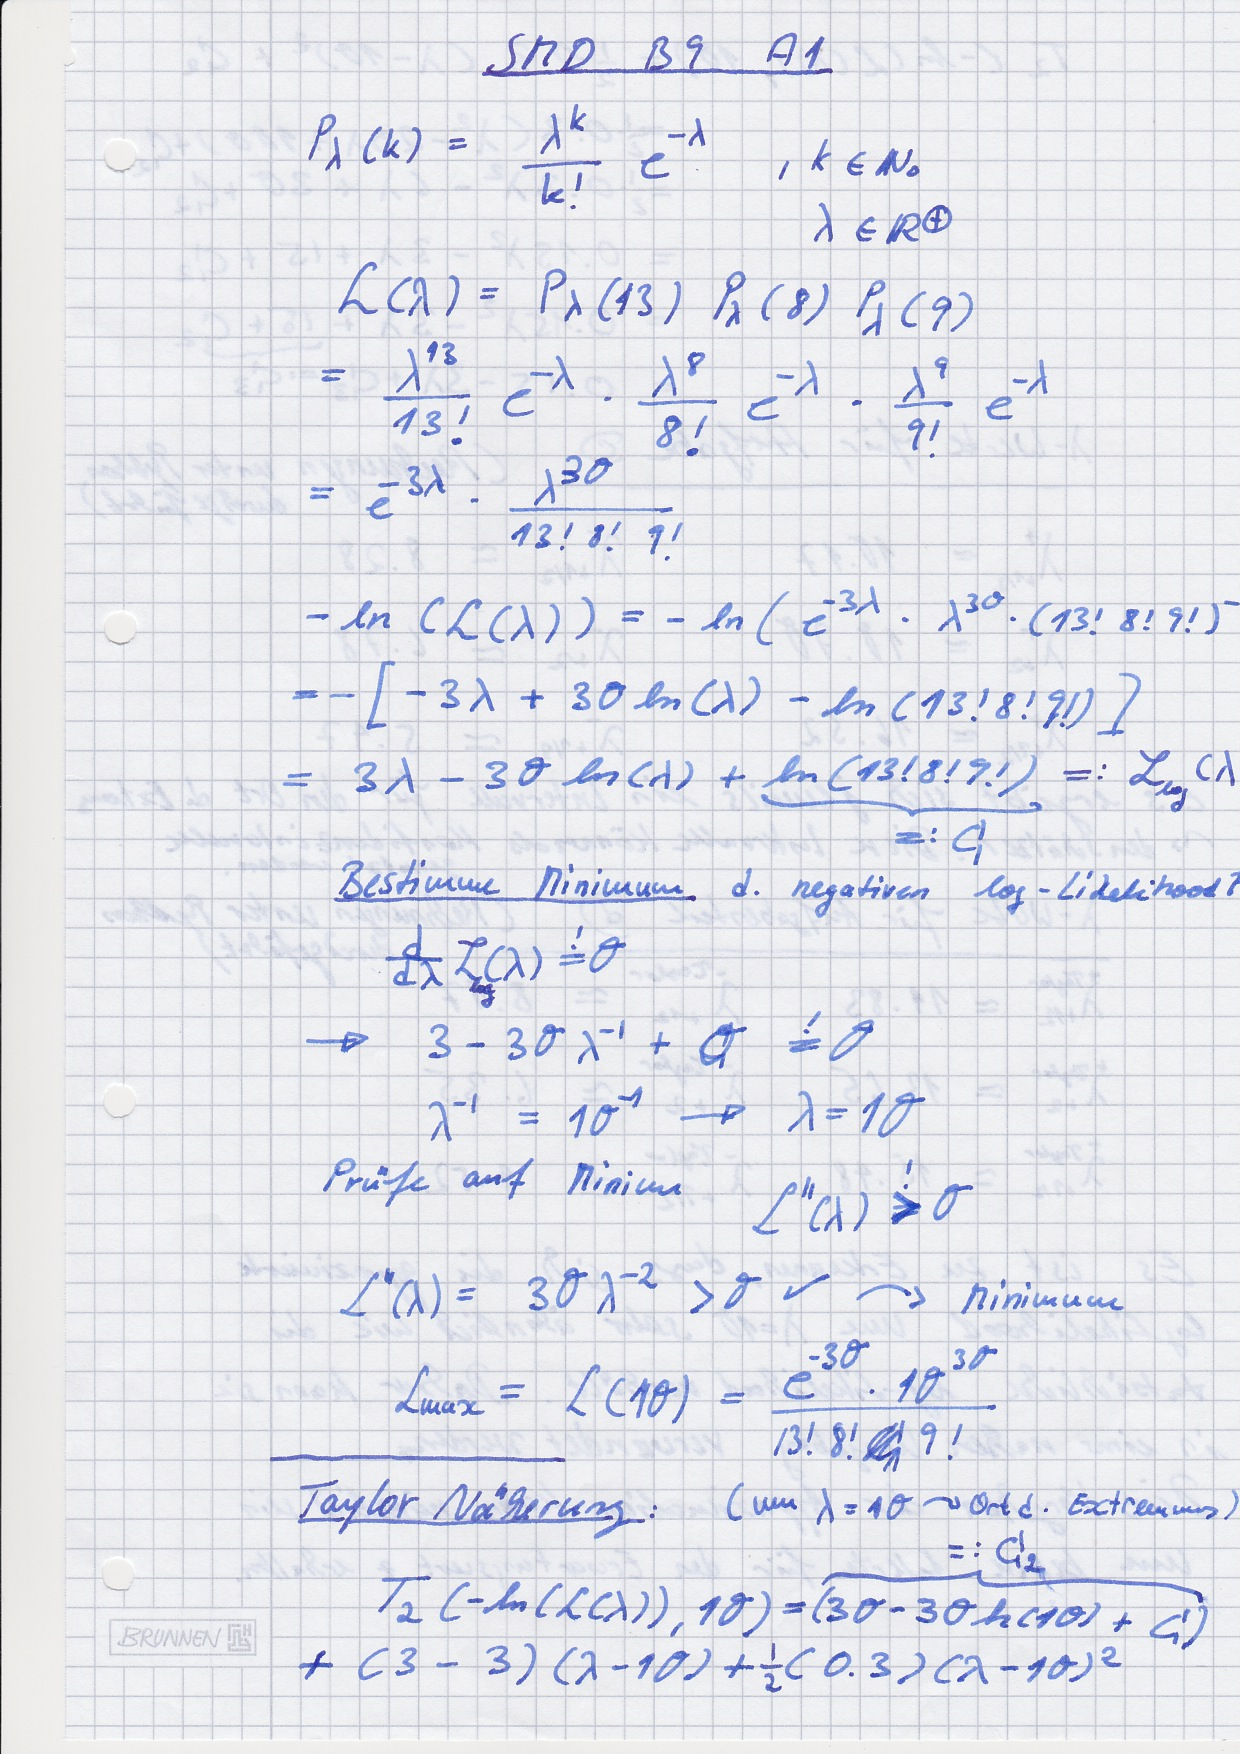
\includegraphics[width=\textwidth]{blatt9p1.jpg}
  \caption{Seite1.}
  \label{fig1}
\end{figure}

\begin{figure}
  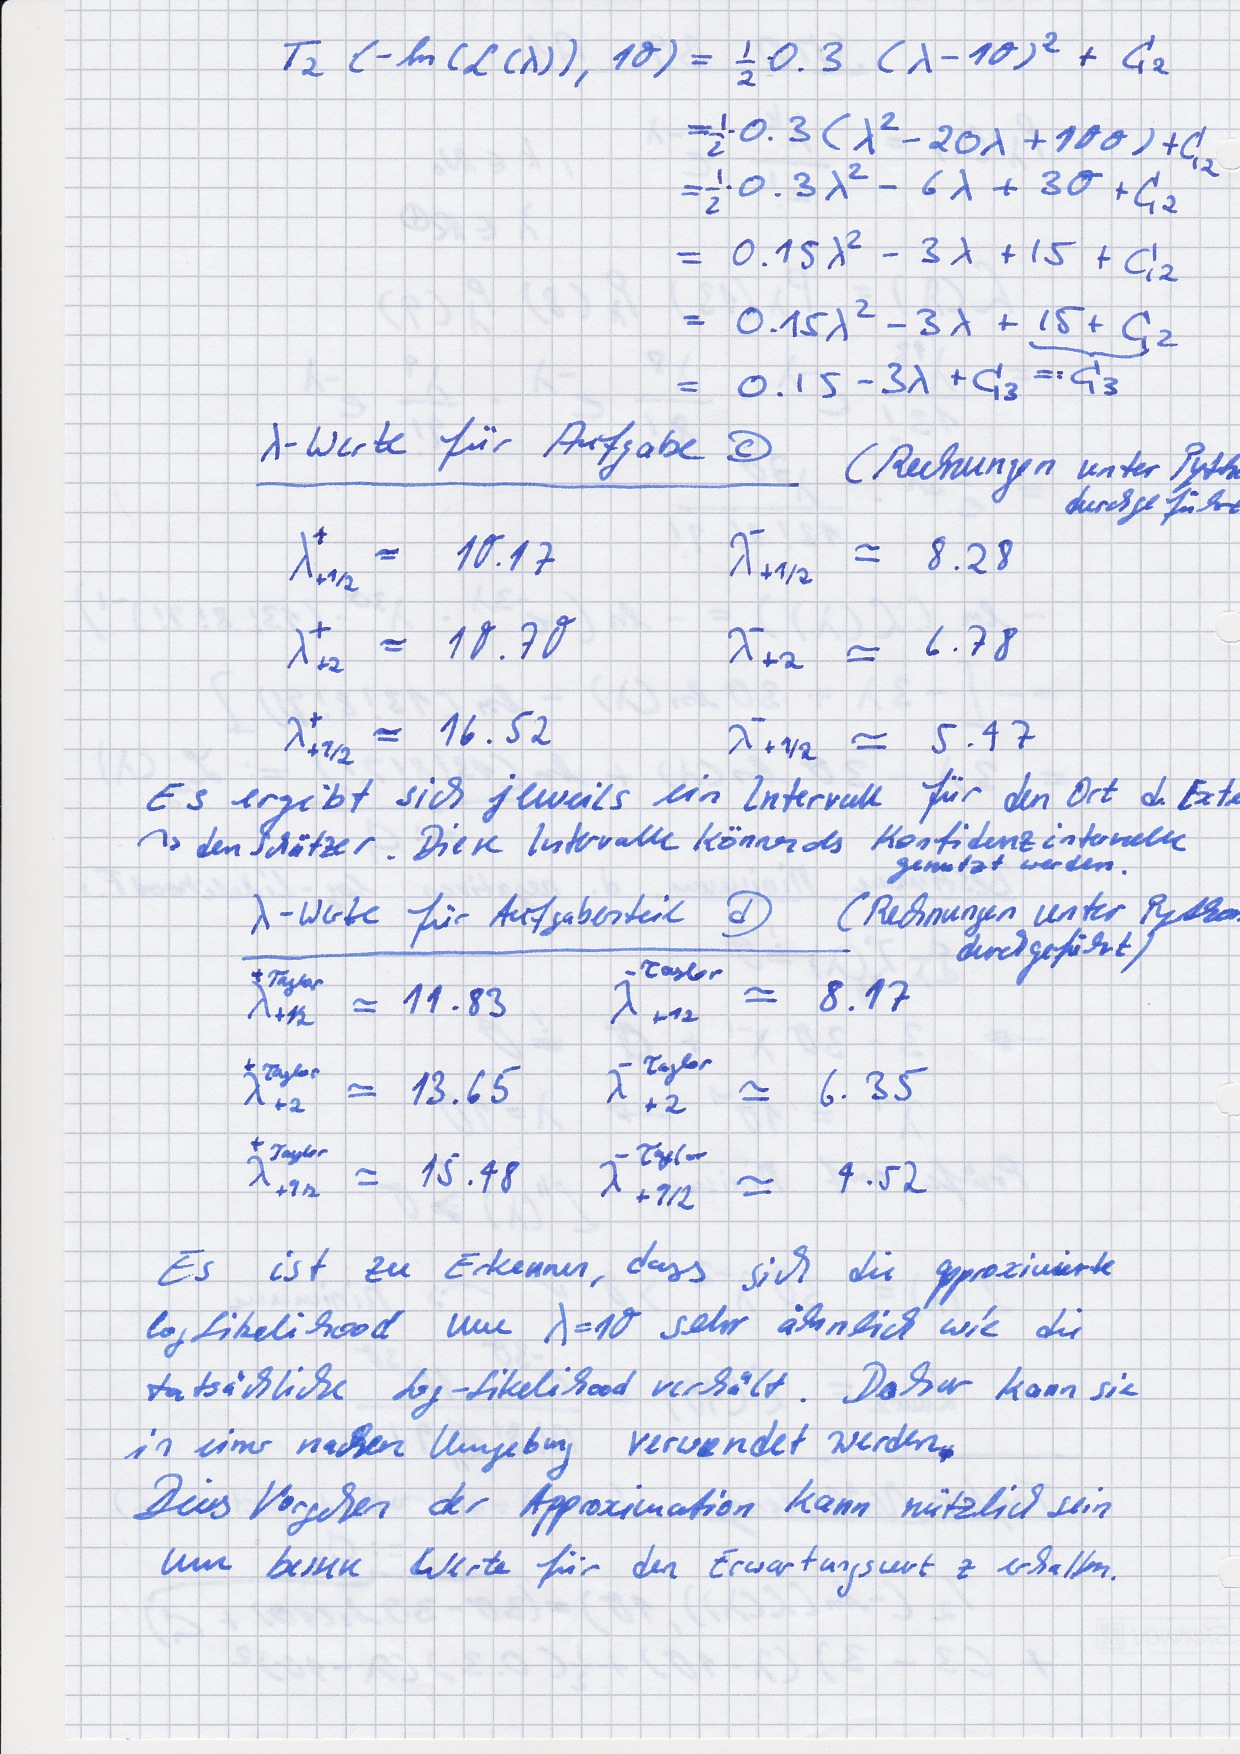
\includegraphics[width=\textwidth]{blatt9p2.jpg}
  \caption{Seite2.}
  \label{fig2}
\end{figure}

\FloatBarrier
\begin{figure}
  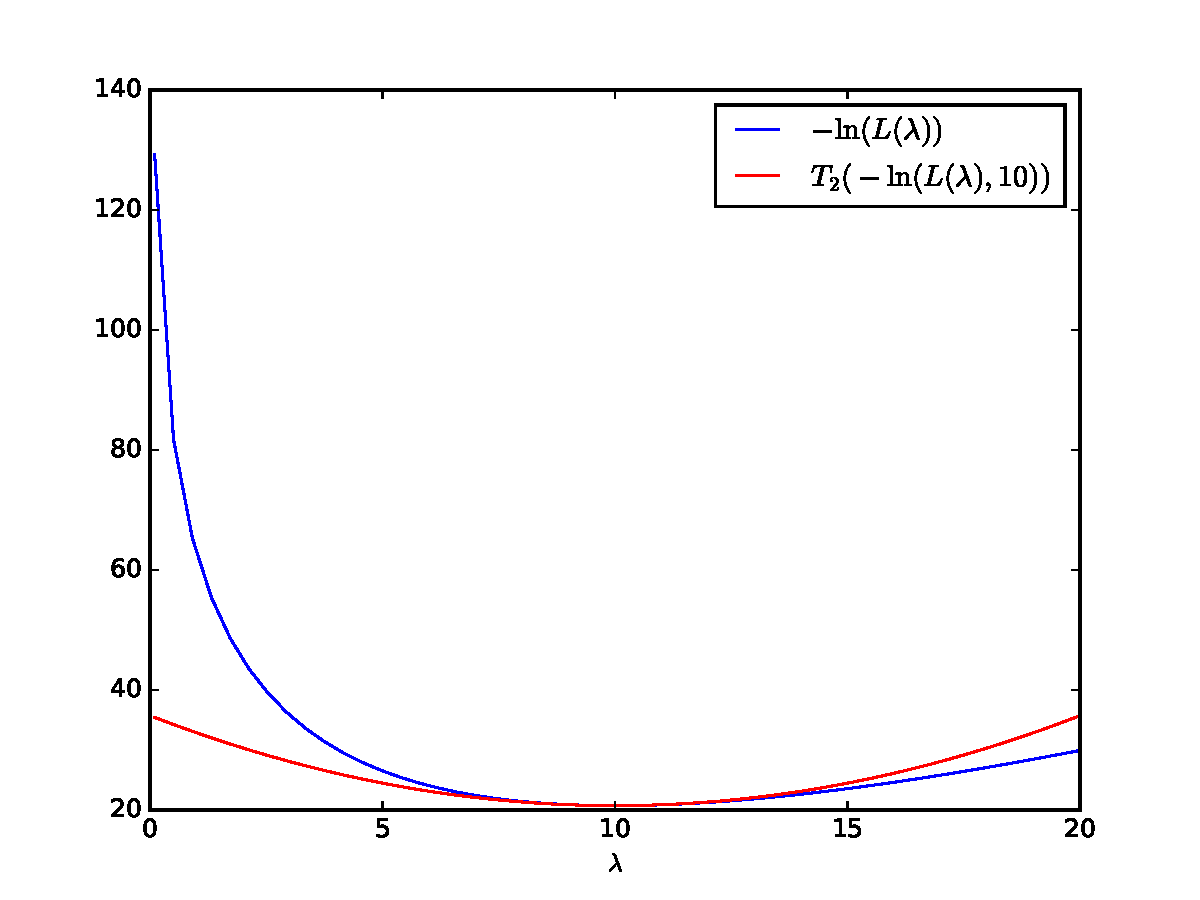
\includegraphics[width=\textwidth]{smdblatt9plot1.pdf}
  \caption{Graphische Darstellung der negativen log-likelihood sowie ihrer Taylornäherung 2.Ordnung.}
  \label{fig3}
\end{figure}

\FloatBarrier
